%!TEX root = mainfile.tex

\section{Introduction} % (fold)
\label{sec:introduction}
This exercise is designed as an introduction to the algorithm used in JPEG compression. Though the actual algorithm that is used is slightly more subtle, this method provides a demonstration of the steps that are used and the effects that they have on the image in question. The effect of each step on the file size of the resulting JPEG image as well as the quality of this image shall be examined.
% section introduction (end) 

\section{JPEG Image Compression} % (fold)
\label{sec:jpeg_image_compression}
The JPEG image format, which stands for the Joint Photographic Experts Group, is a commonly used method of lossy compression used to store images in smaller file sizes whilst sacrificing as little important image information as possible. The information to be removed is chosen based on a consideration of the limitations of the human visual system thereby reducing file size while making little or no noticeable change to perceivable image quality.

There is some uncertainty regarding the origins of the specification for the JPEG format. It is claimed that the original patent outlining the image format was submitted in 1986. The JPEG committee is of the opinion that these claims are not valid and there have been numerous other claims to the ownership and subsequent royalties from the distribution of images stored and distributed in this format. Though the JPEG format is due to remain proprietary, the JPEG committee is aiming to provide it without licence fee after the release of the updated specification JPEG 2000.

Only the first JPEG specification shall be examined, since the methods and algorithms are simpler, though not as efficient as later versions.
% section jpeg_image_compression (end)

\section{Discrete Cosine Transformation (DCT)} % (fold)
\label{sec:discrete_cosine_transformation_}
The method used to compress images in the JPEG format involves taking the Discrete Cosine Transformation (DCT) of the image. 

\subsection{Mathematical Basis} % (fold)
\label{sub:mathematical_basis}
The Discrete Cosine transform converts an input signal, $g(u)$, into a series of coefficients, each representing a different frequency. Given a signal, sampled at $M$ regular intervals, $u=0,1,2\ldots M-1$, the DCT basis function is defined as
\begin{align}
	D_m^M(u) &= c_m \sqrt{\frac{2}{M}}\cos\left(\frac{\pi m(2u+1)}{2M}\right), \qquad m=0\ldots M-1.
\end{align}
where $c_m=\frac{1}{\sqrt 2}$ for $m=0$ and 1 otherwise. These basis functions are orthonormal, and so the scalar product can be taken of them with the original signal, such that the $M$ values of $g(u)$ are transformed into $M$ coefficients, $G(m)$, and the final DCT of $g(u)$ is given by,
\begin{align}
	G(m) &= \sum_{u=0}^{M-1} g(u) D_m^M(u).
\end{align}
By inverting this process, the original signal can be retrieved from the coefficients of the DCT, i.e.\ the signal is given by,
\begin{align}
	g(u) &= \sum_{m=0}^{M-1} G(u) D_m^M(u).
\end{align}
Since this method shall be applied to an image, which is effectively a two dimensional signal, the two dimensional DCT is used,
\begin{align}
	G(m,n) &= \sum_{u=0}^{M-1}\sum_{v=0}^{N-1} g(u,v) D_m^M(u)D_n^N(u).
\end{align}
This two dimensional version is the equivalent of simply taking two successive DCT's, one in the vertical and a second in the horizontal directions. In the context of image processing, this means using a signal comprising a column of pixels and performing the DCT for each column across the image and then taking a row and performing it for each row down the image.
% subsection mathematical_basis (end)

% The exact details of this transform will not be examined here, but it has the effect of splitting a wave-function down into the component frequencies, much as the Fourier Transform does, though providing only real, as opposed to imaginary or complex, results. The results of a discrete cosine transform on a set of data is a number of coefficients that describe the relative intensities of each of the available frequencies. This analysis is carried out on the image in both the horizontal and vertical directions which means that an array of values describing how the frequencies are concentrated about the image can be generated. To easily visualise this, the intensity value can be interpreted as pixel brightness value and so an image, of the same dimensions, can be drawn which is the DCT of the original.
Overall, this has the effect of splitting a wave-function down into the component frequencies, much as the Fourier Transform does, though providing only real, as opposed to imaginary or complex, results. The results of a discrete cosine transform on a set of data is a number of coefficients that describe the relative intensities of each of the available frequencies. To easily visualise this, the intensity value can be interpreted as pixel brightness value and so an image, of the same dimensions, can be drawn which is the DCT of the original.

\subsection{Compression Ratio} % (fold)
\label{sub:compression_ratio}
As a way of applying quantitative scientific methods to the algorithms used to compress images, a value known as the compression ratio is used to compare the results of different methods or aggressiveness of compression. This is simply given by equation \ref{eq:compressratio}.
\begin{align}
	\text{Compression Ratio} &= \frac{\text{Compressed Size}}{\text{Uncompressed Size}} \label{eq:compressratio}
\end{align}
This produces a fraction, the smaller this fraction is, i.e.\ the closer it is to zero, the more space is saved by using that compression on the file.

Another useful value is the space savings provided by a particular compression of a file. This is defined as the reduction in size relative to the uncompressed size and is shown in equation \ref{eq:spacesaving},
\begin{align}
	\text{Space Saving} &= \frac{\text{Uncompressed Size} - \text{Compressed Size}}{\text{Uncompressed Size}} \\
	 &= 1- \frac{\text{Compressed Size}}{\text{Uncompressed Size}} \label{eq:spacesaving}
\end{align}
% subsection compression_ratio (end)

\subsection{Comparison Image} % (fold)
\label{sub:comparison_image}
In order to examine the effects of increasing the compression ratio, an original image shall be used that will not be changed. This image is shown below. It is a 256\,pixel by 256\,pixel 8-bit image saved in the TIFF lossless image format.
\begin{figure}[ht]
 	\centering
 	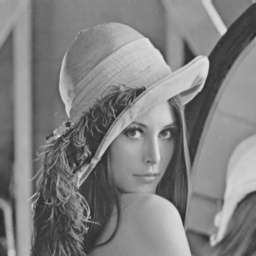
\includegraphics[width=0.5\textwidth]{lena.jpg}
	\caption{The reference image that will be used as a comparator. It is saved using JPEG compression with a quality value of 100\%.\label{fig:orig}}
\end{figure}
This image is then saved as a JPEG file using a quality value of 100\%, i.e.\ as high a quality as possible, in theory losing no information. This resulting file has a size of 37\,386\,bytes (37\,Kb). 
% subsection comparason_image (end)

\subsection{Effect of JPEG Quality Values on Image File Size and Quality} % (fold)
\label{sub:effect_of_jpeg_quality_values_on_image_file_size_and_quality}
A simple examination of the effect of changing the JPEG quality value will demonstrate the range of qualities of the saved file, as well as the size of that file.

The table below, table \ref{fig:percent_vs_size}, shows how the file size of the generated JPEG file changes as the quality value is changed. The quality value is represented as a percentage, and so the range is displayed over the full range from 100\%, being the highest quality possible by the format, to 0\%, being the highest compression ratio and thus the lowest quality.
\begin{figure}[ht]
	\centering
	\begin{minipage}[c]{0.3\linewidth}
		\centering
	 	\begin{tabular}{C{4.4em}|C{3.7em}}
			Quality Value (\%) 	& File Size (bytes) \\
			\hline \hline
			100 & 37\,386 \\
			% 98 & 29\,035 \\
			% 95 & 20\,972 \\
			% 93 & 17\,567 \\
			90 & 14\,868 \\
			% 85 & 11\,943 \\
			80 & 10\,289 \\
			% 75 & 9076 \\
			70 & 8364 \\
			% 65 & 7703 \\
			60 & 7142 \\
			% 55 & 6705 \\
			50 & 6313 \\
			% 45 & 5989 \\
			40 & 5589 \\
			% 35 & 5226 \\
			30 & 4782 \\
			% 25 & 4331 \\
			20 & 3823 \\
			% 15 & 3305 \\
			10 & 2367 \\
			% 5 & 1863 \\
			0 & 1407 \\
		\end{tabular}
	\end{minipage}
	\begin{minipage}[c]{0.65\linewidth}
		\centering
		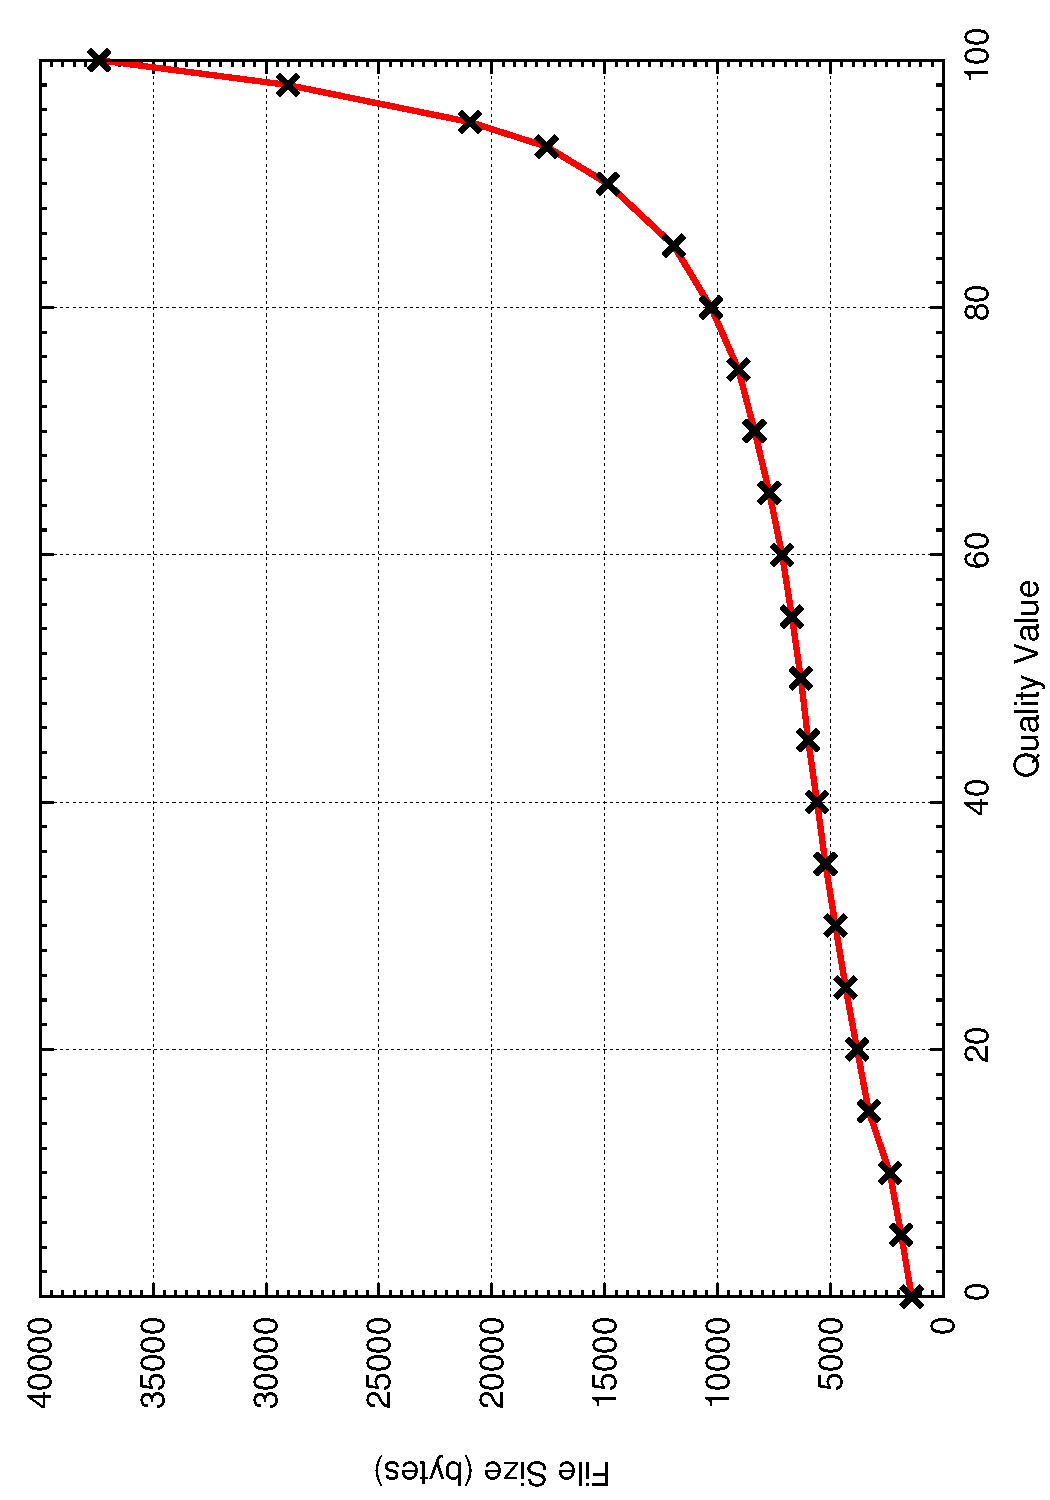
\includegraphics[angle=270,width=\textwidth]{qualityvsfilesize.pdf}
	\end{minipage}
	\caption{The file size of a JPEG image increases as the quality of the encoding increases, so that less information is left out from the original image.\label{fig:percent_vs_size}}
\end{figure}

As can be seen, the relation is approximately linear for quality values up to roughly 80\% and then the file size increases more quickly. For comparison, the same image, when saved in the TIFF format, has a file size of 65\,684\,bytes, so even the ``100\%'' quality JPEG file is a factor of 1.76 times smaller, a compression ratio of 0.57. Though there are large savings in the space taken to store the image when the high compression is used, there are noticeable changes as visual artefacts start to become apparent as the compression is increased. This effect can be seen in the images in figure \ref{fig:various_lena}.

\begin{figure}[ht]
	\centering
	\begin{minipage}[c]{0.19\linewidth}
		\centering
	 	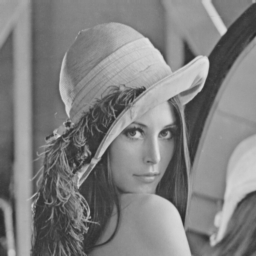
\includegraphics[trim = 20mm 30mm 40mm 30mm, clip]{lena256x256_100.jpg}
	\end{minipage}
	\begin{minipage}[c]{0.19\linewidth}
		\centering
	 	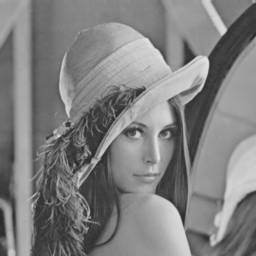
\includegraphics[trim = 20mm 30mm 40mm 30mm, clip]{lena256x256_70.jpg}
	\end{minipage}
	\begin{minipage}[c]{0.19\linewidth}
		\centering
	 	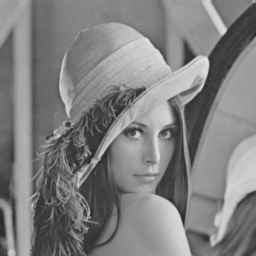
\includegraphics[trim = 20mm 30mm 40mm 30mm, clip]{lena256x256_40.jpg}
	\end{minipage}
	\begin{minipage}[c]{0.19\linewidth}
		\centering
	 	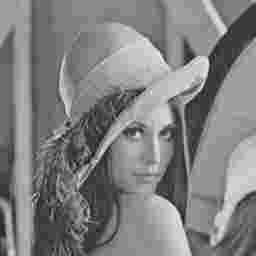
\includegraphics[trim = 20mm 30mm 40mm 30mm, clip]{lena256x256_10.jpg}
	\end{minipage}
	\begin{minipage}[c]{0.19\linewidth}
		\centering
	 	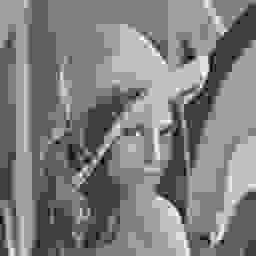
\includegraphics[trim = 20mm 30mm 40mm 30mm, clip]{lena256x256_00.jpg}
	\end{minipage}
	\caption{Since the JPEG compression algorithm involves removing information from the image in order to reduce its file size, the quality of the image degrades as the compression ratio is increased. The first image shows a zoomed section of the picture after minimal compression has been applied. This image has the largest file size. Each of the next three images represent the same image with a compression of 30\% less than the previous, i.e.\ 70\%, 40\%, and 10\%. The final image shows the effect of the maximum compression, minimum file size, with a quality of 0\% where serious image degradation is observed and the image is almost unrecognisable.\label{fig:various_lena}}
\end{figure}
% subsection effect_of_jpeg_quality_values_on_image_file_size_and_quality (end)

\section{Disregarding Sections of the DCT} % (fold)
\label{sec:disregarding_sections_of_the_dct}
The algorithm that is used for JPEG compression involves removing some of the high frequency components of the image. The DCT of an image orders the frequency components, increasing from the lowest to the highest in both the horizontal and vertical directions. Thus, if the bottom right section of the DCT, i.e.\ the high frequency region, is removed, then the total information required to describe the resulting inverse DCT image is reduced and so the file size is decreased. 

The level to which this can be performed is dependant only on what the human eye can perceive and the ``importance'' of the resulting image. This means that, if the final image is going to be used only as a small picture on a website for example, a lot of information can be lost without noticeable difference, but if the image is a photograph to be printed, then the difference will be much more noticeable. It is this compromise that must be decided when changing the JPEG quality value.

\subsection{Performing the DCT Using Block Sizes} % (fold)
\label{sub:performing_the_dct_using_block_sizes}
Since the discrete cosine transform involves mathematically comparing every pixel with all those nearby, performing it on a large image very quickly becomes time consuming and computationally intensive. To reduce this, with little difference in the image quality or file compression ratio, the DCT is performed on 8 by 8 pixel sections of the image separately and then this array of DCT results is combined to get a tiled $N$ by $N$ composite, where $N$ is the number of 8 by 8 blocks that are required to make up the full image.

The image below, figure \ref{fig:lena_DCT} shows the results of the DCT on the original image. The shapes of the original image are just perceivable since each 8 by 8 block has areas of high complexity, represented by whiter colours, that correspond to areas of interest in the original, figure \ref{fig:orig}, such as transition from foreground to background etc.
% \begin{figure}[ht]
% 	\centering
% 	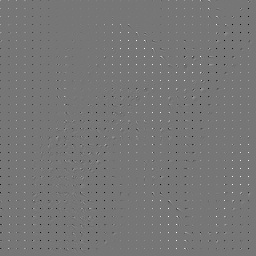
\includegraphics[width=0.5\textwidth]{DCT_lena.jpg}
% 	\caption{A representation of the 256 by 256\,pixels tiled DCT image composed of 32 by 32 times 8 by 8 blocks each of which represent the DCT of a small section of the original image.\label{fig:lena_DCT}}
% \end{figure}
\begin{figure}[ht]
	\centering
	\begin{minipage}[c]{0.45\linewidth}
		\centering
	 	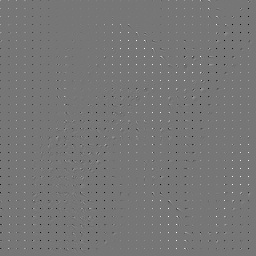
\includegraphics[width=\textwidth]{DCT_lena.jpg}
	\end{minipage}
	\begin{minipage}[c]{0.45\linewidth}
		\centering
	 	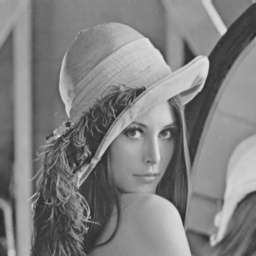
\includegraphics[width=\textwidth]{lena.jpg}
	\end{minipage}
	\caption{A representation of the 256 by 256\,pixels tiled DCT image composed of 32 by 32 times 8 by 8 blocks each of which represent the DCT of a small section of the original image.\label{fig:lena_DCT}}
\end{figure}
% subsection performing_the_dct_using_block_sizes (end)

\subsubsection{Manual JPEG Compression - Frequency Removal} % (fold)
\label{sub:manual_jpeg_compression_frequency_removal}
In order to manually perform the compression that is achieved algorithmically by JPEG compatible programs, some of the higher frequency elements of the DCT shall be removed by using an image ``mask''. This is simply an array of 1's or 0's in the pattern desired, which is multiplied with the image in question so that where there was a 1 in the mask, no change is made, but where there was a 0, the image pixel value is reduced to 0. This mask will then be applied to the DCT results and the inverse DCT taken to reveal the newly compressed image. 

Since it is high frequencies that are required to be removed, and in the DCT these are located toward the bottom right corner, the mask that shall be used comprises 1's in the top left and 0's in the bottom right, as shown in figure \ref{fig:mask}. Now, this mask represents the values that shall be multiplied with the DCT image to compress it, but only for a singe 8 by 8 block. Since the DCT is performed on $N$ by $N$ blocks, it is necessary to have $N$ by $N$ of these masks, figure \ref{fig:NxN_mask}.
\begin{figure}[ht]
	\centering
	\begin{minipage}[c]{0.45\linewidth}
		\centering
	 	
\includegraphics[width=0.5\textwidth]{mask.jpg}
	 	\caption{A single image mask for an 8 by 8 block of the image.\label{fig:mask}}
	\end{minipage}
	\begin{minipage}[c]{0.45\linewidth}
		\centering
	 	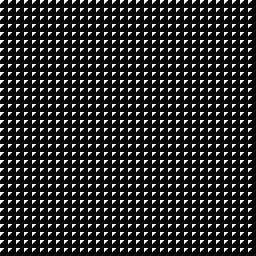
\includegraphics[width=0.6\textwidth]{NxN_mask.jpg}
	 	\caption{When combined together, the total image mask will remove a substantial amount of information from the DCT.\label{fig:NxN_mask}}
	\end{minipage}
\end{figure}

This DCT mask image and the original DCT are multiplied together and then an inverse DCT is taken of this new reduced DCT array. The resulting compressed image is shown below, figure \ref{fig:mancompresslena}.
\begin{figure}[ht]
	\centering
	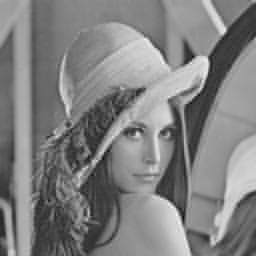
\includegraphics[width=0.5\textwidth]{lena_manual_compression.jpg}
	\caption{A manually compressed image using the same compression method as that used in JPEG encoding.\label{fig:mancompresslena}}
\end{figure}

As can be seen, the image quality has decreased, suggesting that some information has indeed been removed from the file. To confirm this, the new file size is 19\,180\,bytes (19\,Kb), which is a reduction in size by a factor of almost 2, a compression ratio of 0.51. This image represents a removal of 54\,pixels out of a possible 64\,pixels, thus a quality value of 15.625\%. This method could be edited to take account of different quality values by simply removing more or less of the DCT frequencies as desired. Removing more of the higher frequencies would result in still smaller files but worse image quality, whereas removing less would improve the quality but also increase the size needed to store it.

% subsection manual_jpeg_compression_frequency_removal (end)
% section disregarding_sections_of_the_dct (end)
\subsection{Addition to the DCT} % (fold)
\label{sub:addition_to_the_dct}
So far, the effects of removing part of the DCT where the higher frequencies lie has been explored. This has the effect of softening the transitions from high to low pixel value, and so reducing complexity of the image. If instead, the lower frequencies are removed, i.e.\ the top left section of the DCT is set to zero and this time the higher frequencies are retained, the opposite effect is observed. Now, the lower frequencies are left out so that regions where the pixels vary slowly from high to low pixel value will instead vary more quickly. This has the reversed effect of ``sharpening'' the image.

Since no information can be added to the image, in fact the total information needed to describe the image has still decreased, no additional detail can be revealed. Instead, details in the image will appear to be more defined though speckling, artefacts and a decrease in accuracy with the original will soon appear. The images in figure \ref{fig:sharp} show this effect when the high frequencies are decreased by different amounts.
\begin{figure}[ht]
	\centering
	\begin{minipage}[c]{0.3\linewidth}
		\centering
	 	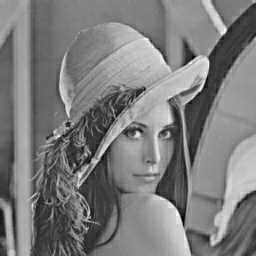
\includegraphics[width=0.9\textwidth]{lena_sharp1.jpg}
	\end{minipage}
	\begin{minipage}[c]{0.3\linewidth}
		\centering
	 	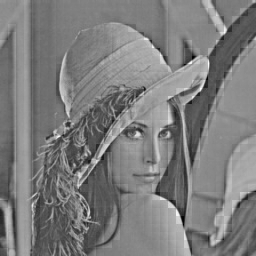
\includegraphics[width=0.9\textwidth]{lena_sharp2.jpg}
	\end{minipage}	
	\begin{minipage}[c]{0.3\linewidth}
		\centering
	 	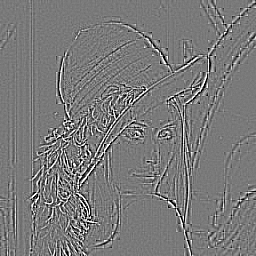
\includegraphics[width=0.9\textwidth]{lena_edge.jpg}
	\end{minipage}
 	\caption{When the low frequencies are reduced in the DCT, the resulting compressed image is said to have been sharpened. Increasing the amount of removal very quickly leads to very poor image quality where only the edges are left since these vary in pixel value most quickly. This has some uses in image processing such as motion detection or OCR (optical character recognition), though more rigorous methods exist, such as the sharpening filter ($1-\nabla^2$), which produce much better results.\label{fig:sharp}}
\end{figure}

Since the sample image is a relatively complex image, much of the information is in these higher frequencies. For this reason, a much reduced version of the previous mask is used so that only the highest frequency element in the 8 by 8 DCT image is reduced, not removed, by a multiplying factor greater than 1.
% subsection addition_to_the_dct (end)
% section discrete_cosine_transformation_ (end)
\section{Conclusion} % (fold)
\label{sec:conclusion}
Since the human eye is less sensitive to rapid changes in brightness in an image, i.e.\ the high frequencies are ``neurologically less important'', these are chosen to be removed when simply compressing an image using JPEG encoding. The actual JPEG algorithm is very similar to the method explained here, though slightly more subtle. Rather than always selecting the same triangular portion of the DCT, it weighs the DCT components from top left to bottom right and then discards the least important ones based on the results.
% section conclusion (end)



%%%%%%%What is file compression ratio?? have you included it?
